\subchapter{Bootloader - U-Boot}{Objectives: Set up serial
  communication, compile and install the U-Boot bootloader, use basic
  U-Boot commands, set up TFTP communication with the development
  workstation.}

As the bootloader is the first piece of software executed by a
hardware platform, the installation procedure of the bootloader is
very specific to the hardware platform. There are usually two cases:

\begin{itemize}

\item The processor offers nothing to ease the installation of the
  bootloader, in which case the JTAG has to be used to initialize
  flash storage and write the bootloader code to flash. Detailed
  knowledge of the hardware is of course required to perform these
  operations.

\item The processor offers a monitor, implemented in ROM, and through
  which access to the memories is made easier.

\end{itemize}

The Xplained board, which uses the SAMA5D3 SoCs, falls into the second
category. The monitor integrated in the ROM reads the MMC/SD card to
search for a valid bootloader before looking at the internal NAND
flash for a bootloader. Whenever nothing's available, it will operate
in a fallback mode, that will allow to use an external tool through
USB to reflash some bootloader. Therefore, either by using an MMC/SD
card or that fallback mode, we can start up a SAMA5D3-based board
without having anything installed on it.

\section{Setup}

Go to the \code{~/felabs-sysdev/bootloader} directory.

If you are using a 64 bit installation of Ubuntu, install support for
executables built with a 32 bit C library:

\begin{verbatim}
sudo apt-get install ia32-libs
\end{verbatim}

We're going to use that fallback mode, and its associated tool,
\code{sam-ba}.

We first need to download this tool, from Atmel's website.

\begin{verbatim}
wget http://www.atmel.com/Images/sam-ba_2.12.zip
unzip sam-ba_2.12.zip
\end{verbatim}

\section{Setting up serial communication with the board}

Plug the Xplained board on your computer using the provided
USB-to-serial cable. When plugged-in, a serial port should appear,
\code{/dev/ttyUSB0}.

You can also see this device appear by looking at the output of
\code{dmesg}.

To communicate with the board through the serial port, install a
serial communication program, such as \code{picocom}:

\begin{verbatim}
sudo apt-get install picocom
\end{verbatim}

You also need to make your user belong to the \code{dialout} group to be
allowed to write to the serial console:

\begin{verbatim}
sudo adduser $USER dialout
\end{verbatim}

You need to log out and in again for the group change to be effective.

Run \code{picocom -b 115200 /dev/ttyUSB0}, to start serial
communication on \code{/dev/ttyUSB0}, with a baudrate of 115200. If
you wish to exit \code{picocom}, press \code{[Ctrl][a]} followed by
\code{[Ctrl][x]}.

\section{AT91Bootstrap Setup}

The boot process is done in two steps with the ROM monitor trying to
execute a first piece of software, called \code{AT91Bootstrap}, from
its internal SRAM, that will initialize the DRAM, load \code{U-Boot}
that will in turn load Linux and execute it.

As far as bootloaders are concerned, the layout of the NAND flash will
look like:

\begin{center}
  \includegraphics[width=\textwidth]{labs/sysdev-u-boot/flash-map.pdf}
\end{center}

\begin{itemize}
\item Offset \code{0x0} for the first stage bootloader is dictated by
  the hardware: the ROM code of the SAMA5D3 looks for a bootloader at
  offset \code{0x0} in the NAND flash.
\item Offset \code{0x40000} for the second stage bootloader is decided
  by the first stage bootloader. This can be changed by changing the
  AT91Bootstrap configuration.
\item Offset \code{0xc0000} of the U-Boot environment is decided by
  U-Boot. This can be changed by modifying the U-Boot configuration.
\end{itemize}

The first item to compile is AT91Bootstrap that you can fetch from
Atmel's github account:

\begin{verbatim}
git clone git://github.com/linux4sam/at91bootstrap.git -b at91bootstrap-3.x
cd at91bootstrap
\end{verbatim}

Then, we first need to configure the build system for our setup. We're
going to need a few informations for this:

\begin{itemize}
\item Which board you want to run AT91Bootstrap on
\item Which device should AT91Bootstrap will be stored on
\item What component you want AT91Boostrap to load
\end{itemize}

You can get the list of the supported board by listing the
\code{board} directory. You'll see that in each of these folder, we
have a bunch of \code{defconfig} files, that are the supported
combinations. In our case, we will load U-Boot, from the NAND.

Then, you've found the right defconfig, load it using
\code{make <defconfig_name>}, and you can start the compilation using
\code{make}\footnote{You can speed up the compiling by using the
  \code{-jX} option with \code{make}, where X is the number of
  parallel jobs used for compiling. Twice the number of CPU cores is a
  good value.}. Don't forget to set the \code{CROSS_COMPILE}
environment variable!

At the end of the compilation, you should have a file called
\code{sama5d3_xplained-nandflashboot-uboot-*.bin}, in the
\code{binaries} folder.

In order to flash it, we need to do a few things. First, remove the
\code{NAND CS} jumper on the board. It's next to the pin header
closest to the Micro-USB plug. Reset the board, and put the jumper
back. On the serial port, you should see \code{RomBoot}.

Then, start \code{sam-ba} as root. You'll get a small window. Select
the \code{ttyACM0} connection, and the \code{at91sama5d3x-ek} board. Hit
\code{Connect}.

You need to:
\begin{itemize}
\item Hit the NANDFlash tab
\item In the scripts choices, select \code{Enable NandFlash} and hit \code{Execute}
\item Select \code{Erase All}, and execute the command
\item Then, select \code{Enable OS PMECC} parameters in order to
  change the NAND ECC parameters to what RomBOOT expects. Change the
  number of ECC bits to 4, and the ECC offset to 36.
\item Finally, send the image we just compiled using the command
  \code{Send Boot File}
\end{itemize}

AT91Bootstrap should be flashed now, keep sam-ba opened, and move to
the next section.

\section{U-Boot setup}

Download U-Boot using git:

\begin{verbatim}
git clone http://git.denx.de/u-boot.git
cd u-boot
\end{verbatim}

We're going to use the latest released version: \code{2014.07-rc2}.

Switch to this version using \code{git checkout v2014.07-rc2}.

Get an understanding of its configuration and compilation steps by
reading the \code{README} file, and specifically the {\em Building the
  software} section.

Basically, you need to:

\begin{itemize}

\item set the \code{CROSS_COMPILE} environment variable;

\item run \code{make <NAME>_config}, where \code{<NAME>} is the name
  of your board as declared in the \code{boards.cfg} file. There are
  two flavors of the Xplained: one to run from the SD card
  (\code{sama5d3_xplained_mmc}) and one to run from the NAND flash
  (\code{sama5d3_xplained_nandflash}). Since we're going to boot on
  the NAND, use the latter. Note that for our platform, both these
  choices are sharing most of their configuration, that is defined in
  \code{include/configs/sama5d3_xplained.h}. Read this file to get an
  idea of how a U-Boot configuration file is written;

\item Finally, run \code{make}, which should build U-Boot.

\end{itemize}

Now, in sam-ba, in the \code{Send File Name} field, set the path to
the \code{u-boot.bin} that was just compiled, and set the address to
\code{0x40000}. Click on the \code{Send File} button.

\section{Testing U-Boot}

Reset the board and check that it boots your new bootloaders. You can
verify this by checking the build dates:

\begin{verbatim}
AT91Bootstrap 3.6.2-00090-g1e8fd41ce714 (mercredi 4 juin 2014, 11:08:41 (UTC+0200))

NAND: ONFI flash detected
NAND: Manufacturer ID: 0x2c Chip ID: 0x32
NAND: Disable On-Die ECC
NAND: Initialize PMECC params, cap: 0x4, sector: 0x200
NAND: Image: Copy 0x80000 bytes from 0x40000 to 0x26f00000
NAND: Done to load image


U-Boot 2014.07-rc2 (Jun 04 2014 - 12:38:09)

CPU: SAMA5D36
Crystal frequency:       12 MHz
CPU clock        :      528 MHz
Master clock     :      132 MHz
DRAM:  256 MiB
NAND:  256 MiB
MMC:   mci: 0
*** Warning - bad CRC, using default environment

In:    serial
Out:   serial
Err:   serial
Net:   gmac0
Warning: failed to set MAC address
, macb0
Warning: failed to set MAC address
\end{verbatim}

Interrupt the countdown to enter the U-Boot shell:
\begin{verbatim}
U-Boot #
\end{verbatim}

In U-Boot, type the \code{help} command, and explore the few commands
available.

\section{Setting up Ethernet communication}

Later on, we will transfer files from the development workstation to
the board using the TFTP protocol, which works on top of an Ethernet
connection.

To start with, install and configure a TFTP server on your development
workstation, as detailed in the bootloader slides.

With a network cable, connect the Ethernet port of your board to the
one of your computer. If your computer already has a wired connection
to the network, your instructor will provide you with a USB Ethernet
adapter. A new network interface, probably \code{eth1} or \code{eth2},
should appear on your Linux system.

To configure this network interface on the workstation side, click on
the {\em Network Manager} tasklet on your desktop, and select {\em
  Edit Connections}.

\begin{center}
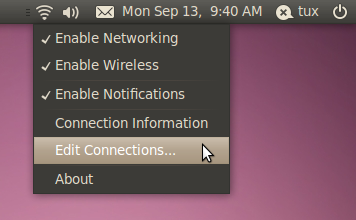
\includegraphics[width=8cm]{labs/sysdev-u-boot/network-config-1.png}
\end{center}

Select the new {\em wired network connection}:

\begin{center}
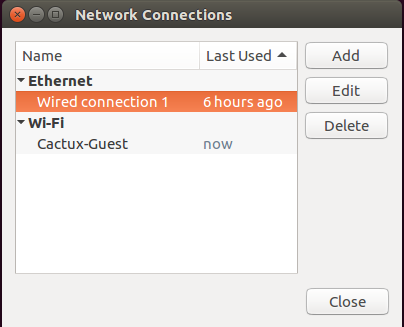
\includegraphics[width=8cm]{labs/sysdev-u-boot/network-config-2.png}
\end{center}

In the \code{IPv4 Settings} tab, press the \code{Add} button
and make the interface use a static IP
address, like \code{192.168.0.1} (of course, make sure that this
address belongs to a separate network segment from the one of the main
company network).

\begin{center}
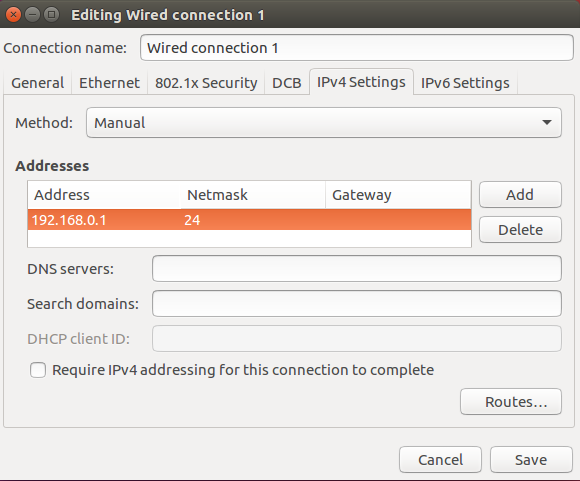
\includegraphics[width=8cm]{labs/sysdev-u-boot/network-config-3.png}
\end{center}

You can use \code{255.255.255.0} as \code{Netmask}, and leave the
\code{Gateway} field untouched (if you click on the \code{Gateway} box, you
will have to type a valid IP address, otherwise you won't be apply to
click on the \code{Apply} button).

Now, configure the network on the board in U-Boot by setting the \code{ipaddr}
and \code{serverip} environment variables:

\begin{verbatim}
setenv ipaddr 192.168.0.100
setenv serverip 192.168.0.1
\end{verbatim}

The first time you use your board, you also need to send the MAC address
in U-boot:

\begin{verbatim}
setenv ethaddr 00:01:02:03:04:05
\end{verbatim}

In case the board was previously configured in a different way, we
also turn off automatic booting after commands that can be used to
copy a kernel to RAM:

\begin{verbatim}
setenv autostart no
\end{verbatim}

To make these settings permanent, save the environment:

\begin{verbatim}
saveenv
\end{verbatim}

Now switch your board off and on again\footnote{Power cycling your
  board is needed to make your \code{ethaddr} permanent, for obscure
  reasons. If you don't, U-boot will complain that \code{ethaddr} is not
  set.}.

You can then test the TFTP connection. First, put a small text file in
the directory exported through TFTP on your development
workstation. Then, from U-Boot, do:

\begin{verbatim}
tftp 0x22000000 textfile.txt
\end{verbatim}

{\bf Caution: known issue in Ubuntu 12.04 and later}:
if this command doesn't work, you may have to stop the server
and start it again every time you boot your workstation:

\begin{verbatim}
sudo service tftpd-hpa restart
\end{verbatim}

The \code{tftp} command should have downloaded
the \code{textfile.txt} file from your development
workstation into the board's memory at location 0x80000000 (this
location is part of the board DRAM). You can verify that the download
was successful by dumping the contents of the memory:

\begin{verbatim}
md 0x22000000
\end{verbatim}

We will see in the next labs how to use U-Boot to download, flash and
boot a kernel.

\section{Rescue binaries}

If you have trouble generating binaries that work properly, or later
make a mistake that causes you to loose your bootloader binaries, you
will find working versions under \code{data/} in the current lab
directory.
